\section{Stochastic Particle Tracing using Particle Filtering}

As presented above, the particle tracing result of a given seed position $x_0$ for the distribution-based data $\mathcal{H}$ can be represented as a pdf $p({v_{0:n}}|{\lambda_{0:n}})$ over the trace domain $\Omega_{x_0}$, which is given by equation (8). However, $p({v_{0:n}}|{\lambda_{0:n}})$ is high-dimensional, non-standard, and only known up to a proportionality constant, which makes it infeasible to be evaluated in closed-form. Therefore, a Monte Carlo based method needs to be used to approximate the target distribution. In this case, particle filtering as one of Sequential Monte Carlo methods is suitable to approximate the target distribution in iterations.

\subsection{Posterior Approximation with Properly Weighted Traces}

\begin{figure}[htb]
  \centering
  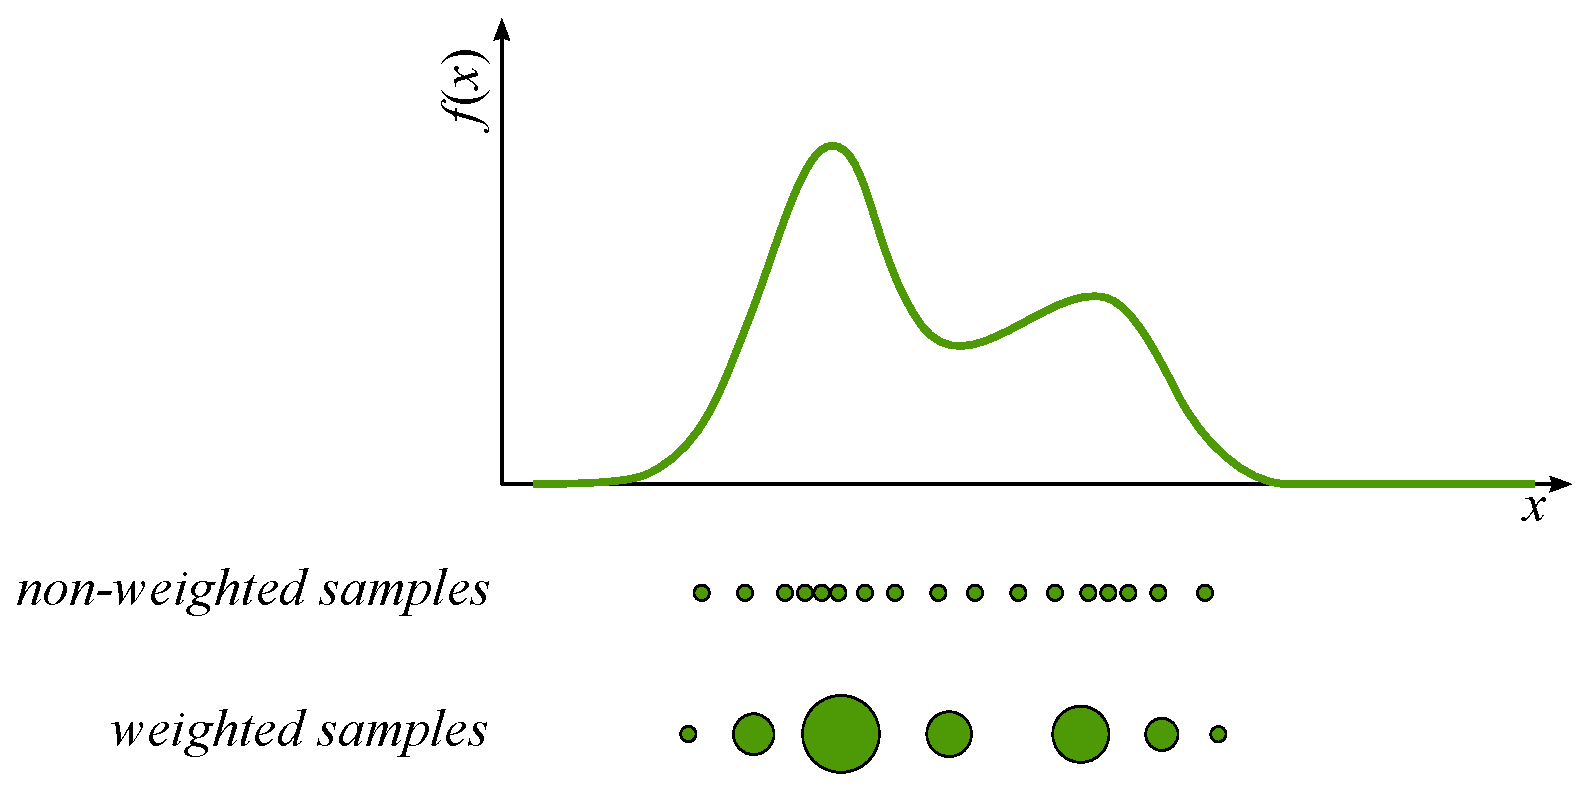
\includegraphics[width=3in]{../figures/importance_sampling.eps}
  \caption{Non-weighted and weighted samples representing the probability density function $f(x)$. Fewer samples is needed to represent the target pdf by using weighted samples.}
  \label{importance_sampling}
\end{figure}

In order to work with the complicated target posterior density $p({v_{0:n}}|{\lambda_{0:n}})$, a more convenient representation is needed to approximate it. By applying the particle filtering method, the target posterior density can be represented by a set of properly weighted traces, which are denoted as $\{ v_{0:n}^i,w_n^i\} _{i = 1}^{{N_s}}$, where $N_s$ is the number of samples and $ w_n^i,i = 0,...,{N_s} $ are the associated weights. Therefore, we can estimate some statistical properties, for example the mean, variance, and maximum likelihood of the target posterior density from the sample traces. Compared to the non-weighted samples used by the conventional Monte Carlo method, weighted samples can represent the target distribution more efficiently. A comparison between weighted and non-weighted samples is illustrated in Figure~\ref{importance_sampling}. A common way of drawing properly weighted samples from the target distribution is to use importance sampling, which samples from a trivial distribution $q({v_{0:n}}|{\lambda_{0:n}})$ called the importance function and assign a weight to each of the random samples according to
\begin{equation}
  w_n = \frac{{p({v_{0:n}}|{\lambda_{0:n}})}}{{q({v_{0:n}}|{\lambda_{0:n}})}}
\end{equation}

\subsection{Sequential Build-Up}

Since the dimension of the target posterior density increases as the number of propagation steps in the particle tracing grows, which makes it difficult to directly obtain the final sample traces with a given step number $n$. By applying particle filtering we smoothly approach the final probability density by building up the sample traces sequentially. To do so, we put ${N_s}$ particles at the seed position $x_0$ and update them iteratively. At each iteration $t$, we have a set of properly weighted samples $\{ v_{0:t-1}^i,w_{t-1}^i\} _{i = 1}^{{N_s}}$ which represents the probability density $p({v_{0:t-1}}|{\lambda_{0:t-1}})$, then each sample can be updated to step $t$ according to the recursive form of the posterior density $p({v_{0:t}}|{\lambda_{0:t}})$, which can be written as:
\begin{equation}
  p({v_{0:t}}|{\lambda_{0:t}}) = p({v_{0:t - 1}}|{\lambda_{0:t - 1}})p(v_t|v_{t-1},\lambda_t)
\end{equation}
where
\begin{equation}
  p(v_t|v_{t-1},\lambda_t) = \frac{{p({\lambda_t}|{v_t})p({v_t}|{v_{t - 1}})}}{{p({\lambda_t}|{\lambda_{0:t - 1}})}}
\end{equation}
Since directly sampling vectors from $p(v_t|v_{t-1},\lambda_t)$ is difficult, we make use of an alternative density function $q({v_t}|{v_{t - 1}},{\lambda_t})$ which is so-call the importance function presented above. From the importance function, vector directions $v_t$ can be obtained, therefore the weights can be updated according to equation (13). Theoretically, the importance function can be any distribution for the vector direction $v_t$. However, a bad choice of the importance function may produce vector directions which have low probability in the target distribution. Hence, the choice of the importance function will influence the performance of the particle filtering algorithm significantly, which will be detailed in the next section. In order to iteratively update the weights on-line, the importance function is chosen to factorize such that:
\begin{equation}
  q({v_{0:t}}|{\lambda_{0:t}}) = q({v_{0:t - 1}}|{\lambda_{0:t - 1}})q({v_t}|{v_{t - 1}},{\lambda_t})
\end{equation}
After getting random vector directions according to the importance density $q({v_t}|{v_{t - 1}},{\lambda_t})$, the weights $\{w_t^i\} _{i = 1}^{{N_s}}$ of traces is updated based on $\{w_{t-1}^i\} _{i = 1}^{{N_s}}$. By substituting (14), (16) into (13), we can get the equation to update the weight:
\begin{equation}
  w_t^i = w_{t - 1}^i\frac{{p({\lambda_t}|v_t^i)p(v_t^i|v_{t - 1}^i)}}{{q(v_t^i|v_{t - 1}^i,{\lambda_t})p({\lambda_t}|{\lambda_{0:t - 1}})}}
\end{equation}
Since the weights can be normalized by:
\begin{equation}
  w_t^i = \frac{{w_t^i}}{{\sum\limits_{j = 1}^{{N_s}} {w_t^j} }}
\end{equation}
the normalizing constant ${p({\lambda_t}|{\lambda_{0:t - 1}})}$ can be ignored. Therefore, the weight update equation can be simplified as
\begin{equation}
  w_t^i \propto w_{t - 1}^i\frac{{p({\lambda_t}|v_t^i)p(v_t^i|v_{t - 1}^i)}}{{q(v_t^i|v_{t - 1}^i,{\lambda_t})}}
\end{equation}

The results provided by the particle filtering algorithm for a given seed position is a set of weighted traces which approximate the posterior probability distribution of the possible traces. We directly render them to see the uncertainty of the particle tracing process. With respect to the goal of visualizing the global phenomenon of the vector fields, streamlines originating from different seed positions need to be visualized together, which make it inappropriate to show all the sample traces for a given seed position all the time. To solve this problem, we extract the trace with highest probability based on the posterior density function and visualize all the most likely traces together. The most likely trace is chosen by maximum a posteriori probability (MAP) estimation, which is the trace with the maximal importance weight.

\subsection{Resampling and Choice of Importance Function}

A common issue with the particle filtering algorithm is the degeneracy problem, which is that after several iterations, some samples will have extremely small weights. This means that the contribution of those samples to the posterior distribution is negligible. A reasonable measurement of degeneracy is the effective sample size $N_{eff}$ introduced in~\cite{Liu98sequentialmonte}, which can be estimated by
\begin{equation}
  {N_{eff}} = \frac{1}{{\sum\limits_{i = 1}^{{N_s}} {{{(w_t^i)}^2}} }}
\end{equation}
where $w_t^i$ is the normalized weight. The value of $N_{eff}$ is between $1$ and $N_s$ and the smaller $N_{eff}$ is, the weights degenerate more. The degeneracy problem is an undesirable effect in particle filters. The brute force approach to reduce this effect is to use a very large sample size, which is often impractical. Hence, we focus on two other methods.

\textbf{Resampling} The first method is to perform resampling~\cite{doucet2001sequential, gordon:107} whenever the degeneracy becomes significant (i.e., when $N_{eff}$ is smaller than some hard threshold $N_t$). The key idea of resampling is to remove the traces that have small weights and duplicate the traces which have large weights. To do so, we generate a new set of weighted traces by resampling (with repalcement) $N_s$ times from the given set $\{ v_{0:t}^i,w_t^i\} _{i = 1}^{{N_s}}$, making use of the weights $\{w_t^i\} _{i = 1}^{{N_s}}$ as the probabilities for a sample to be resampled, then reset the weights to $w_t^i = \frac{1}{{{N_s}}}$.

\textbf{Good Choice of Importance Function} The second method is choosing a good importance density $q({v_t}|{v_{t - 1}},{\lambda_t})$. The optimal importance density function that minimizes the variance of the weights $w_t^i$ conditioned on $v_{t-1}$ and $\lambda_t$, pointed out by Doucet et al. in~\cite{Doucet00onsequential}, is $p(v_t|v_{t-1}, \lambda_t)$. However, this optimal importance density requires the evaluation of the integral over the new state, which makes it difficult to sample efficiently from. Hence, we focus on designing a suboptimal importance density which can be easily sampled from and represents $p(v_t|v_{t-1}, \lambda_t)$ well. A usual approach is to use the same distribution as the prior density as the importance function, which is called bootstrap filter or condensation algorithm. However, such importance function may not be always effective, since no observation information is used. As a result, the resulting particles are often outliers of the posterior distribution. Therefore, the observation density is used to determine the $v_t$. Since it is expensive to evaluate the observation density function and there is no need to use the actual observation density as the importance density for the particle filtering method, we choose the observed distribution $\lambda_t$ as the importance density function.

\subsection{Algorithm Summary}

Our stochastic particle tracing algorithm is summarized in Algorithm~\ref{algo:pf}.

\begin{algorithm}[h]
\caption{Streamline Estimation with Particle Filtering} \label{algo:pf}
\begin{algorithmic} [1]

\State Let $x_0$ be a given seed position, $n$ be the number of steps, $N_s$ be the number of samples.
\For {$t=0:n$}
\For {$i=1:N_s$}
\State Sample $v_t^i$ at position $x_t$ according to ${\lambda_t}$
\State Compute weight $w_t^i$ according to (11), (12), and (19)
\EndFor
\State Normalize the weights $\{w_t^i\}_{i=1}^{N_s}$ according to (18)
\State Calculate $N_{eff}$ using (20)
\If {$N_{eff} < N_t$}
\State Resample $\{ v_{0:t}^i,w_t^i\} _{i = 1}^{{N_s}}$ to obtain $N_s$ equally-weighted particles $\{ \hat{v}_{0:t}^i,\frac{1}{N_s}\} _{i = 1}^{{N_s}}$
\EndIf
\State Propagate $x_t$ to $x_{t+1}$ according to (1)
\EndFor

\end{algorithmic}
\end{algorithm}
